\documentclass[a4paper]{article}
\usepackage{amsmath}
\usepackage{amsthm}
\usepackage{amssymb}
\usepackage{pifont}
\usepackage{listings}
\newtheorem{thm}{Theorem}
\usepackage[english]{babel}
\usepackage[utf8]{inputenc}
\usepackage{graphicx}
\usepackage[colorinlistoftodos]{todonotes}
\setlength{\parskip}{8pt}
\setlength{\parindent}{0pt}

\usepackage{graphicx}
\graphicspath{{../images/}}

\lstset{language=Python,
    basicstyle=\ttfamily,
    showstringspaces=false,
}

\newcommand{\xmark}{\ding{55}}%
\newcommand{\cmark}{\ding{51}}%
\newcommand{\inlinecode}{\texttt}

\title{Introduction to Python}

\author{}
\date{}
\begin{document}
\maketitle

\section{Introduction}

The purposes of this course are:

\begin{itemize}
  \item Learn computational models of thinking.
  \item Master the art of computational problem solving.
  \item Make computers do what you want them to do.
\end{itemize}

\subsection{What does a computer do?}

Fundamentally, a computer does only two things:

\begin{enumerate}
  \item It performs calculations.
  \item It remember results.
\end{enumerate}

One might be wondering how fast a computer performs calculations, so nowadays
a computer can perform approximately a billion calculations per second.
On the other hand, nowadays computers have a hard drive of nearly 1 TB which
means that a computer can store approximately 1.5 million books of standard
size.

\subsection{What kind of operations does a computer perform?}

Every computer comes with a set of built-in operations. These are typically
primitive arithmetic operations such as addition, multiplicaton, division, and
simple logic operations such as comparing true and false values in order make
decisions.

Because this built-in tools are not enough, in this course one will learn how
to define new calculations, new operations, and give them to the computer, so
it can abstract them, encapsulate them, and treat them as they are primitives.

\subsection{Simple calculations and storage enough?}

It is very important to design good algorithms since simple taks could take
a lot of time, and results could required a lot of space to be storaged.
For example, searching on the world wide web using simple operations could take
5.2 days, or deciding a chess move without an optimal algorithm could take 30
minutes.

Considering the same chess problem, experts suggest that there are
approximately $10^{123}$ different possible games. However, there are only
$10^{80}$ atoms in the observable universe. Hence, it is simply not
possible to store all different possible games in chess.

\subsection{Are there limits?}

Despite its speed and size, a computer has limitations. For instance, some
problems are still too complex such as accurate weather prediction and
cracking encryption schemes, or some ploblems are fundamentally impossible to
compute as the famous Halting problem which basically asks to predict whether
a piece of code will always halt with an answer for any input.

\section{Types of Knowledge}

It is possible to divide knowledge into two types:

\begin{enumerate}
  \item \textit{Declarative knowledge:} it is statements of fact, i.e., statements of
        truth.
  \item \textit{Imperative knowledge:} it is a recipe, i.e., how-to knowlege or how-to
        information. It gives a sequence of steps to find a solution.
\end{enumerate}

Both kind of knowledge are important, but only the second one allows getting
the computer to do something.

\subsection{A numerical example}
\textit{Declarative knowledge:} the square root of a number $x$ is $y$ such
that $y * y = x$. The previous sentence is a statement of fact. Though it is
not telling how to find a square root, it is telling how to check if a number
is the square root of another one.

\textit{Imperative knowledge:} Heron of Alexandria's algorithm to find the
square root of a number $x$ (e.g. 16):

\begin{enumerate}
  \item Start with a guess, $g$.
  \item If $g * g$ is close enought to $x$, then stop and say $g$ is the
        answer.
  \item Otherwise, make a new guess by averaging $g$ and $x/g$.
  \item Using the new guess, repeat process until close enough.
\end{enumerate}


\begin{table}[h!]
\begin{center}
  \begin{tabular}{|p{2.0cm}|p{2.0cm}|p{2.0cm}|p{2.0cm}|}
    \hline
    $g$ & $g * g$ & $x / g$ & $(g + x / g) / 2$\\
    \hline
    3 & 9 & 5.333 & 4.1667\\
    \hline
    4.1667 & 17.36 & 3.837 & 4.0035\\
    \hline
    4.0035 & 16.0277 & 3.997 & 4.000002\\
    \hline
  \end{tabular}
\caption{Heron's algorithm to find the square root of 16.}
\end{center}
\end{table}

\subsection{What is a recipe?}

A recipe has:

\begin{enumerate}
  \item A sequence of simple steps.
  \item A flow of control, a process that specifies when each step is executed.
  \item A way to decide when to stop.
\end{enumerate}

The previous three pieces constitute what is known as an algorithm.

\section{Machines}

One might be wondering how to capture a recipe or algorithm in a mechanical
process. Historically, there have been two options. The former is to use what
is called as a \textit{fixed program computer}, i.e., a computer specifically
designed to calculate a particular computation. For example, handheld
calculators have been fixed to do addition, subtraction, multiplication this
is simple set of arithmetic operations, and that's all they can do.

The alternative to a fixed program computer is a \textit{stored program
computer}. One can load into this computer an algorithm, and inside of it, a
set of parts are going to execute those instructions whenever one wants.
Inside a stored program computer there is a special program known as the
interpreter which is going to walk through each of those sequence of
instructions doing the required computation. The advantage is that now one can
load any algorithm without the need of having to build another computer to run
the new program.

\subsection{Basic Machine Architecture}

Basically, a machine has memory which a place where to store information.
This information could be data but it also can be a sequence of instructions
that constitute an algorithm. A machine will also have a way to load things
into it and to print data out of it, i.e., input and output.

Inside the heart of the machine there are two elements. The former is called
A.L.U. (Arithmetic Logic Unit) which takes information from memory, reads it
in to do perform a primitive operation (as addition or multiplication), and
then it will store stuff back up into memory. The latter is called control
unit which keeps track of the specific operation that has to be
computed in the A.L.U. at each point in time.

Inside the control unit there is an important element called program counter.
When loading a program into a machine, the program counter points to the
location of the first instruction. When one asks the machine to execute the
program, the program counter reads that first instruction, so it will cause an
operation to take place, and it will also add one to the program counter which
is going to take it to the next instruction in the sequence and repeat the
process. At some point, a test might be reached, and the value of this test is
going to change the program counter. Eventually, something is going to indicate
to stop the program.

\begin{figure}[h!]
  \centering
  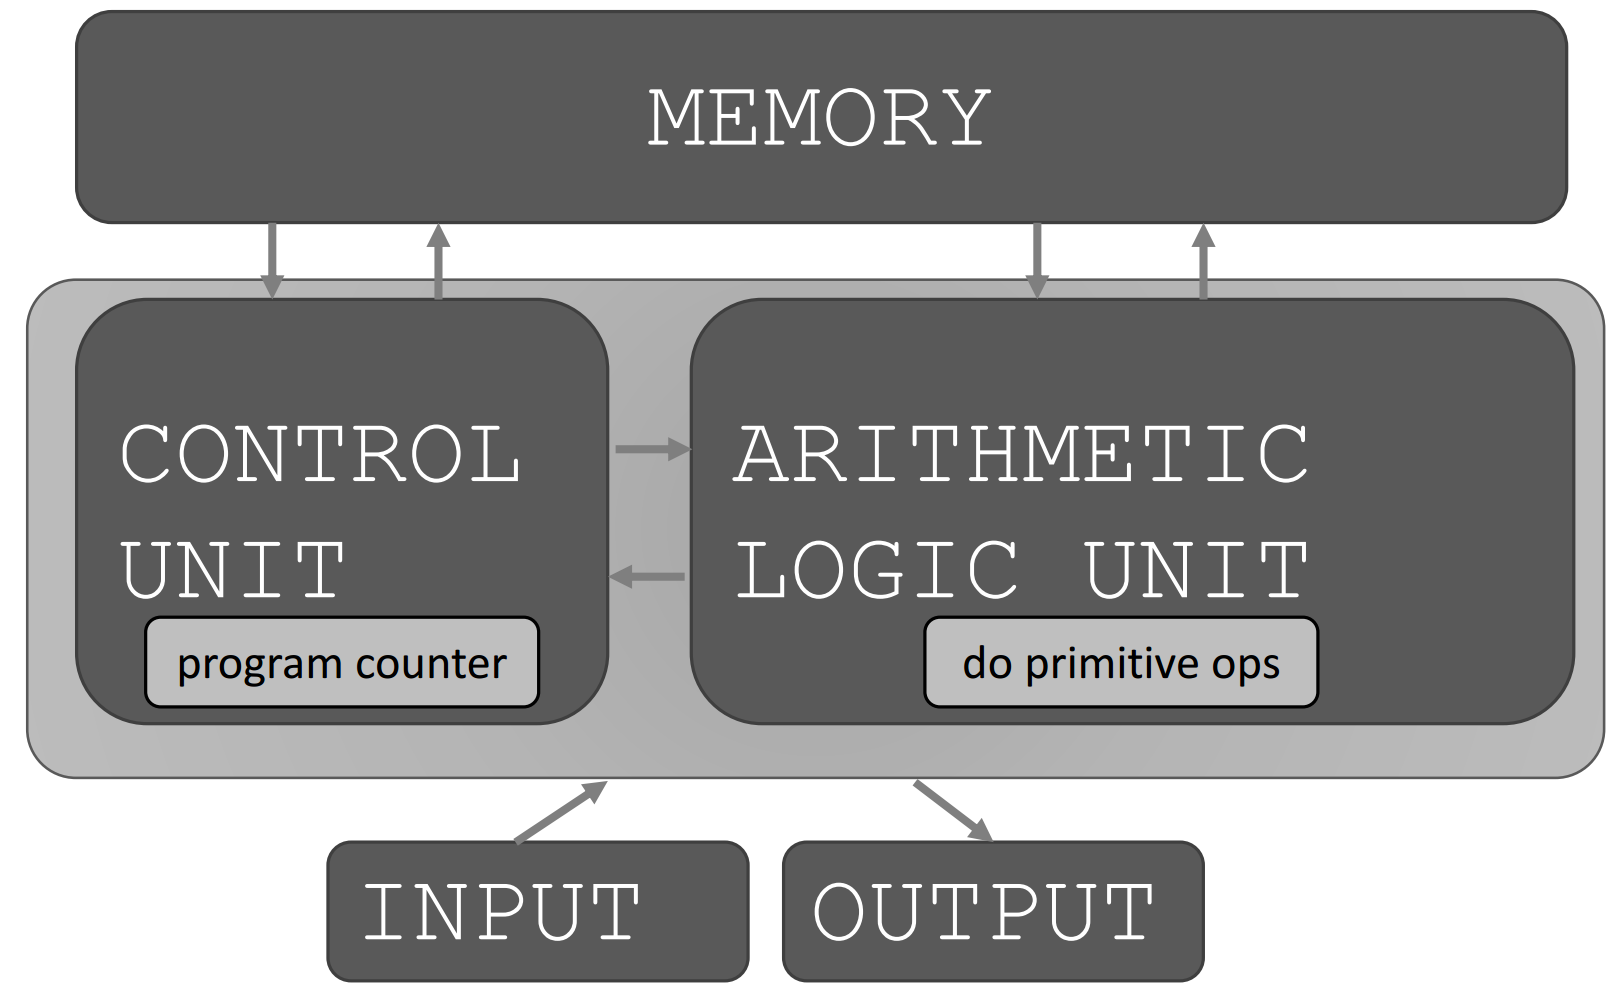
\includegraphics[width=0.5\textwidth]{machine_architecture.png}
  \caption{Basic Machine Architecture}
\end{figure}

\subsection{Stored Program}

A stored program is a sequence of instructions which is built out of simple
arithmetic instructions, logic instructions and simple tests, and it also
allows moving data around. This program has associated with it a special
program called the interpreter which is going to execute each of those
sequences of instructions in order according to the flow of control, and it
will also terminate the program when indicated.

\subsection{Basic Primitives}

Most machines come with simple arithmetic and logic operations, but it is
possible to go simpler than this. Alan Turing showed that one can compute
anything just with six primitives this principle is known as Turing
completeness. In fact, there is something called a Turing machine that is an
infinite tape with a set of squares on it. In each square, there is a symbol
that could be either 0 or 1.

What Turing showed is that if you have six operations and those are: move left,
move right, print, scan, erase, and do nothing, one can compute anything
that is computable. Fortunately, programming languages come with a more
convinient set of primitives, but the fundamental idea is that
\textit{with a simple set of primitives, one is able to compute anything}.

The power of computational thinking relies on being able to write descriptions,
i.e., to abstract methods in order to create new primitives. There is a
fundamental property that says that anything that is computable in one
programming language is computable in another programming language. What is
different is that some taks could be easily done in some programming languages
than in others. This is also a proof of Turing completeness.

\section{Languages}

\subsection{Creating Recipes}

A programming language provides a set of primitive operations, and the next
step is to put them together. In order to to that, one uses expressions which
are complex but legal combinations of primitives. Any legal expression in a
programming language, any computation, has associated with it a value.

\subsection{Aspects of Languages}

While in natural languages such as English the primitive constructs are words,
in a programming language the primitive constructs are \textit{numbers},
sequences of characters a.k.a. \textit{strings}, and \textit{simple operations}
such as addition, subtraction, and comparison.

Once again, when having those primitives, one has to put them together
considering both syntax and semantics. \textit{Syntax} tells whether or not an
expression or combination of expresions is legal. Associated with every
expression that is syntactically valid is the meaning a.k.a semantics.
On one hand, \textit{static semantics} tells which syntactically valid expression
have meaning. On the other hand, \textit{semantics} is the meaning associated
with that syntactically correct string of symbols with no semantic errors.
In order to clarify these three concepts \textit{syntaxis, static semantics}
and \textit{semantics} see table \ref{table:languages}.

\begin{table}[!h]
\begin{center}
  \begin{tabular}{|p{4.5cm}|p{1.50cm}|p{1.8cm}|p{1.75cm}|}
    \hline
    Sentence & Syntaxis & Static Sem. & Semantics\\
    \hline
    I have a dog. & \cmark & \cmark & \cmark\\
    \hline
    Tim saw Jay with a telescope. & \cmark & \cmark & \xmark\\
    \hline
    I are hungry & \cmark & \xmark & no eval\\
    \hline
    cat dog boy & \xmark & no eval & no eval\\
    \hline
  \end{tabular}
\caption{Syntaxis vs. static semantics vs semantics}
\label{table:languages}
\end{center}
\end{table}

Though in English it is possible to have multiple meaning for a sentence,
as in the sentence \textit{Tim saw Jay with a telescope}, in programming
languages an expression has only one meaning. However, the meaning could be not
the one that me programmer intended.

\subsection{Where Things Go Wrong}

Even when a programmer keeps in mind sintaxis, static semantics and semantics,
things can go wrong. For example, he can encounter \textit{syntactic errors}
which are common but easy to find since most programming languages provide a
way to catch them. In addition, a programmer might encounter \textit{static
semantic errors}, i.e., things that they are in the right order, but they
don't make sense. Some programming languages check for them before running a
program, but other languages, as Python, do it on the fly.

The bigger problem is when there are no semantic errors, but the programmer
gets a different meaning than what he expected. There different possible
consequences such as the program can crash or stop running, the program can
run forever, or even worse, the program gives an answer that is different than
the expected.

\section{Types}

As it has been previously mentioned, a program is a sequence of \textit{
definitions} and \textit{commands}. Defitions means ways of either assigning
names to values or more importantly creating procedures that will be treated
as if they are primitives. Commands are simpler expressions that can be
executed directly within Python using the shell which briefly speaking is a
window into which one can type expressions that are passed to the Python
interpreter and prints out the result.

\subsection{Objects}
One of the fundamental primitives in Python are \textit{objects}. Objects
represent data, and programs manipulate objects in order to get out data of
them or do something with them. Every object has a type associated with it,
and this type tells programs whether or not they can act on it.

Objects could be either \textit{scalar} objects or \textit{non-scalar} objects.
Scalar objects cannot be subdivided, and non-scalar objects have internal
structure into which a programmer can pull out parts.

\subsection{Scalar Objects in Python}

There are very few scalar objects in Python:

\begin{itemize}
  \item \inlinecode{int} - represent integers as 9
  \item \inlinecode{float} - represent real numbers as 3.1415
  \item \inlinecode{bool} - represent boolean values as \inlinecode{True} or
        \inlinecode{False}
  \item \inlinecode{NoneType} - special one that has just one value
        \inlinecode{None}
\end{itemize}

It is possible to use \inlinecode{type()} to see the type of an object.

\begin{lstlisting}
In [1]: type(9)
Out[1]: int

In [2]: type(3.1415)
Out[2]: float

In [3]: type(True)
Out[3]: bool

In [4]: type(False)
Out[4]: bool

In [5]: type(None)
Out[5]: NoneType
\end{lstlisting}

\subsection{Type Conversion}

It is possible to convert an object of one type to another. This is called
casting.

\begin{lstlisting}
In [1]: float(9)
Out[1]: 9.0

In [2]: type(float(9))
Out[2]: float

In [3]: int(3.1415)
Out[3]: 3

In [4]: type(int(3.1415))
Out[4]: int
\end{lstlisting}

Notice that in Python when casting from \inlinecode{float} to \inlinecode{int}
the decimal part is truncated.

\subsubsection{Printing to the console}

It is possible to use the console or shell to evaluate expressions, but
sometimes the programmer might want to print an expression, so he can use
\inlinecode{print()}.

\begin{lstlisting}
In [1]: 3 + 2
Out[1]: 5

In [2]: print(3 + 2)
5
\end{lstlisting}

Notice that when printing something there is no output since no value is
returned. \inlinecode{print} returns \inlinecode{None}.

\subsubsection{Expressions}

In order to form expressions, which have a value which has a type, objects and
operator must be combined. The following is the syntax for a simple expression.

\begin{lstlisting}
<object> <operator> <object>
\end{lstlisting}

\subsubsection{Operators on \inlinecode{int}s and \inlinecode{float}s}

Considering that \inlinecode{i} and \inlinecode{j} are either an
\inlinecode{int} or a \inlinecode{flaot}, these are the available operators:

\begin{itemize}
  \item \inlinecode{i + j} $\longrightarrow$ the sum of \inlinecode{i} and
        \inlinecode{j}
  \item \inlinecode{i - j} $\longrightarrow$ the difference of \inlinecode{i}
        and \inlinecode{j}
  \item \inlinecode{i * j} $\longrightarrow$ the product of \inlinecode{i} and
        \inlinecode{j}
  \item \inlinecode{i / j} $\longrightarrow$ the division of \inlinecode{i} and
        \inlinecode{j}
  \item \inlinecode{i // j} $\longrightarrow$ the integer division of
        \inlinecode{i} and \inlinecode{j}
  \item \inlinecode{i \% j} $\longrightarrow$ the remainder when\inlinecode{i}
        is divided by \inlinecode{j}
  \item \inlinecode{i ** j} $\longrightarrow$ the \inlinecode{j}-th power of
        \inlinecode{i}
\end{itemize}

\begin{lstlisting}
In [1]: 3 - 2
Out[1]: 1

In [2]: 3 - 2.0
Out[2]: 1.0

In [3]: 3 / 2
Out[3]: 1.5

In [4]: 3 // 2
Out[4]: 1

In [5]: 5 % 3
Out[5]: 2
\end{lstlisting}

When both \inlinecode{i} and \inlinecode{j} have the same type, the result of
the sum, difference, multiplication or power is of this type, but when mixing
an \inlinecode{int} and a \inlinecode{float} the result is a
\inlinecode{float}. The result of a division is always a \inlinecode{float},
while the result of the integer division is an \inlinecode{int} which is the
quotient of that division.

\subsubsection{Simple Operations}

Parentheses are used to tell Python do this operation first. In addition,
there is an operator precedence which are perform in the following order.

\begin{itemize}
  \item \inlinecode{**}
  \item \inlinecode{*},  \inlinecode{/}, and \inlinecode{//}
  \item \inlinecode{+} and \inlinecode{-}
\end{itemize}

Operators at the same level have the same precedece, so when having multiple
operators of the same level they are evaluated from left to right.

\begin{lstlisting}
In [1]: 3 + 2 * 2
Out[1]: 7

In [2]: 3 * 10 / 2
Out[2]: 15.0

In [3]: 2 + 1 - 10
Out[3]: -7

In [4]: 9 // 2 * 4
Out[4]: 16

In [5]: 4 + 7 % 3
Out[5]: 5

In [6]: 5 * (1 + 3)
Out[6]: 20
\end{lstlisting}

\section{Variables}

\subsubsection{Binding variables and values}

In Python, we do an assignment using an equal sign.

\begin{lstlisting}
x = 1.234567
\end{lstlisting}

In the previous piece of code, a variable \inlinecode{x} is being assigned
a value 1.234567. This statement is basically binding or associating with the
name \inlinecode{x} the value 1.234567, and now it is possible to use
\inlinecode{x} wherever one would want by typing \inlinecode{x}.

\subsection{Abstracting Expressions}

Values of expressions are given a name for several reasosn. For example, one
can reuse the name without redoing the computation to obtain the value, or
it makes code easier to understand. In adittion, it makes code easier to
change later.

\begin{lstlisting}
pi = 3.141592
radius = 2.2
area = pi * radius ** 2
\end{lstlisting}

\subsection{Programming vs. Math}

In programming expressions are not like math expressions, i.e., one does not
solve for $x$. In Python, one can add a comment, a line that is completely
ignored by the interpreter, using the number sign or hash \inlinecode{\#}.

\begin{lstlisting}
# This is a comment
pi = 3.141592
radius = 1
# area of a circle
area = pi * radius ** 2
radius = radius + 1 # this is the same as radius += 1
\end{lstlisting}

An assigment statement find the value on the right hand side of the expression,
then take the name on the left and assign that name to that value.

\subsubsection{Changing Bindings}

It is possible to rebind a variable name in a new assignment statement. The
previous value may still be around in memory, but it's lost, i.e., there is
no way to get to it.

\begin{figure}[h!]
  \centering
  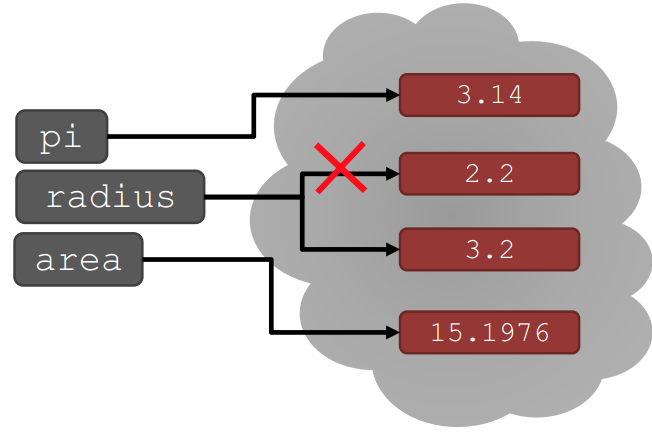
\includegraphics[width=0.6\textwidth]{binding.png}
  \caption{Changing a variable value}
\end{figure}

\begin{lstlisting}
pi = 3.1415
radius = 2
area = pi * radius ** 2
radius += 1
\end{lstlisting}

In the previos suite of code, a suite of code the Pythonic way to call a block
of code, the value for \inlinecode{area} does not change until one tells the
computer to do the calculation again.

\section{Operators and Branching}

\subsection{Comparison Operators on \inlinecode{int} and \inlinecode{float}}

If \inlinecode{i} and \inlinecode{j} are either a \inlinecode{float} or an
\inlinecode{int}, the following comparison operators can be applied,

\begin{itemize}
  \item \inlinecode{i > j} it is evaluated to \inlinecode{True} if
        \inlinecode{i} is greater than \inlinecode{j}.
  \item \inlinecode{i >= j} it is evaluated to \inlinecode{True} if
        \inlinecode{i} is greater than or equal to \inlinecode{j}.
  \item \inlinecode{i < j} it is evaluated to \inlinecode{True} if
        \inlinecode{i} is less than \inlinecode{j}.
  \item \inlinecode{i <= j} it is evaluated to \inlinecode{True} if
        \inlinecode{i} is less than or equal to \inlinecode{j}.
  \item \inlinecode{i == j} it is evaluated to \inlinecode{True} if
        \inlinecode{i} is equal to \inlinecode{j}.
  \item \inlinecode{i != j} it is evaluated to \inlinecode{True} if
        \inlinecode{i} is not equal to \inlinecode{j}.
\end{itemize}

\subsection{Logic Operators on \inlinecode{bool}s}

If \inlinecode{a} and \inlinecode{b} are any variable names:

\begin{itemize}
  \item \inlinecode{not a} $\longrightarrow$ \inlinecode{True} if
        \inlinecode{a} is \inlinecode{False} or \inlinecode{False} if
        \inlinecode{a} is \inlinecode{True}.
  \item \inlinecode{a and b} $\longrightarrow$ \inlinecode{True} if both are
        \inlinecode{True}.
  \item \inlinecode{a or b} $\longrightarrow$ \inlinecode{True} if either or
        both are \inlinecode{True}.
\end{itemize}

\subsection{Branching Programs}

The simplest branching statement is a \textit{conditional}:

\begin{itemize}
  \item A test which is an expression that evalues to either \inlinecode{True}
  or \inlinecode{False}
  \item A block of code to execute if the test is \inlinecode{True}.
  \item A block of code to execute if the test is \inlinecode{False}.
\end{itemize}

In Python, it is not necessary to have the \inlinecode{False} block. It is
mandatory to have the \inlinecode{True} block.

\begin{lstlisting}
x = int(input('Enter an integer: '))

if x % 2 == 0:
    print('Even')
else:
    print('Odd')
print('Done with conditional')
\end{lstlisting}

In Python, indentation is very important not only because it tells which pieces
of code are associated together, but also because not providing indentation
will generate an error. This is different in other programming languages such
as C/C++ or Java in which indentation is only used for readability purposes.

\subsubsection{Nested Conditionals}

It is possible to have nested conditionals, i.e., a conditional inside another
one.

\begin{lstlisting}
if x % 2 == 0:
    if x % 3 == 0:
        print('Divisible by 2 and 3')
    else:
        print('Divisible by 2 and not by 3')
elif x % 3 == 0:
    print('Divisible by 3 and not by 2')
\end{lstlisting}

\subsection{Compound Booleans}

As it has been previously mentioned, it is possible to combine booleans,

\begin{lstlisting}
if x < y and x < z:
    print('x is least')
elif y < z:
    print('y is least')
else:
   print('z is least')
\end{lstlisting}

\subsection{Control Flow - Branching}

Basically in branching, a condition is evaluated and this value is either
\inlinecode{True} or \inlinecode{False}, then a suite of code is evaluated
depending of this value. Figure \ref{img:branching_flow} shows the possible
ways to use branching in Python.

\begin{figure}
  \centering
  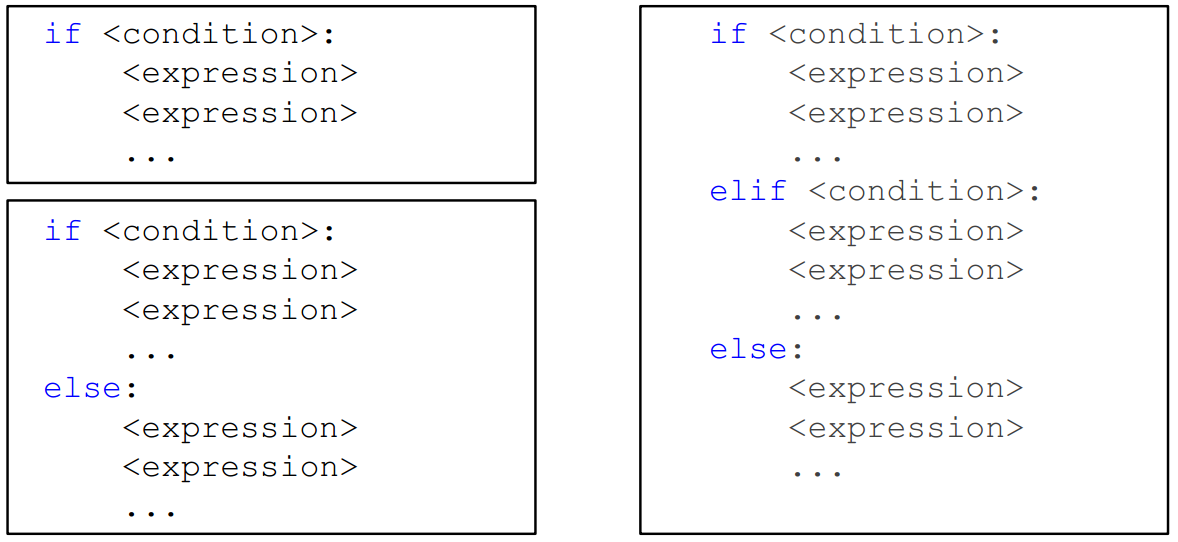
\includegraphics[width=0.9\textwidth]{branching_flow.png}
  \caption{Control flow of branching}
  \label{img:branching_flow}
\end{figure}

To sum up, branching programs allow making choices and do different things, but
each statement is executed at most once. This means that the maximum time to
run the program depends only on the length of the program. As a consequence,
these are the so-called linear programs because they run in constant time,
i.e., each instruction is executed at most once. However, they do not provide
the power to really build interesting algorithms.

\end{document}
